\chapter{Plan}

The plan involves of the following steps, which are elaborated upon in the Gantt Chart seen in Table \ref{fig:plan-gantt-chart}.

\begin{enumerate}
	\item Initial infrastructure setup. This involves building the train-validate-test loops, building the data ingest/transformation pipelines, and building the model-building pipelines. This is feasible in the given timespan since much of the code will be taken from the IRIS Seminar project.
	\item Integration of all modules as well as integration of hyperparameter optimization and training-tracking code complete. Initial training/debugging of the network can begin.
	\item Parallelization of reinforcement-learning and deep-learning components of the network are complete. This involves making it possible to run the RL and the DL models on separate computers during training, if this improves performance.
	\item Get initial results, bugs will be found and ``beta-testing'' of the framework starts. All results at this point are taken with a massive grain of salt since something will cause the results to be wrong, speaking from experience.
	\item Deeper investigations through hyperparameter optimization and changes to the model architecture should now start or is already ongoing.
	\item Final results from the experiments should be completed.
	\item First draft of the paper.
	\item Second draft the paper.
	\item Final draft of the paper.
	\item Thesis defense preparation.
\end{enumerate}

\begin{figure}
	\centering
	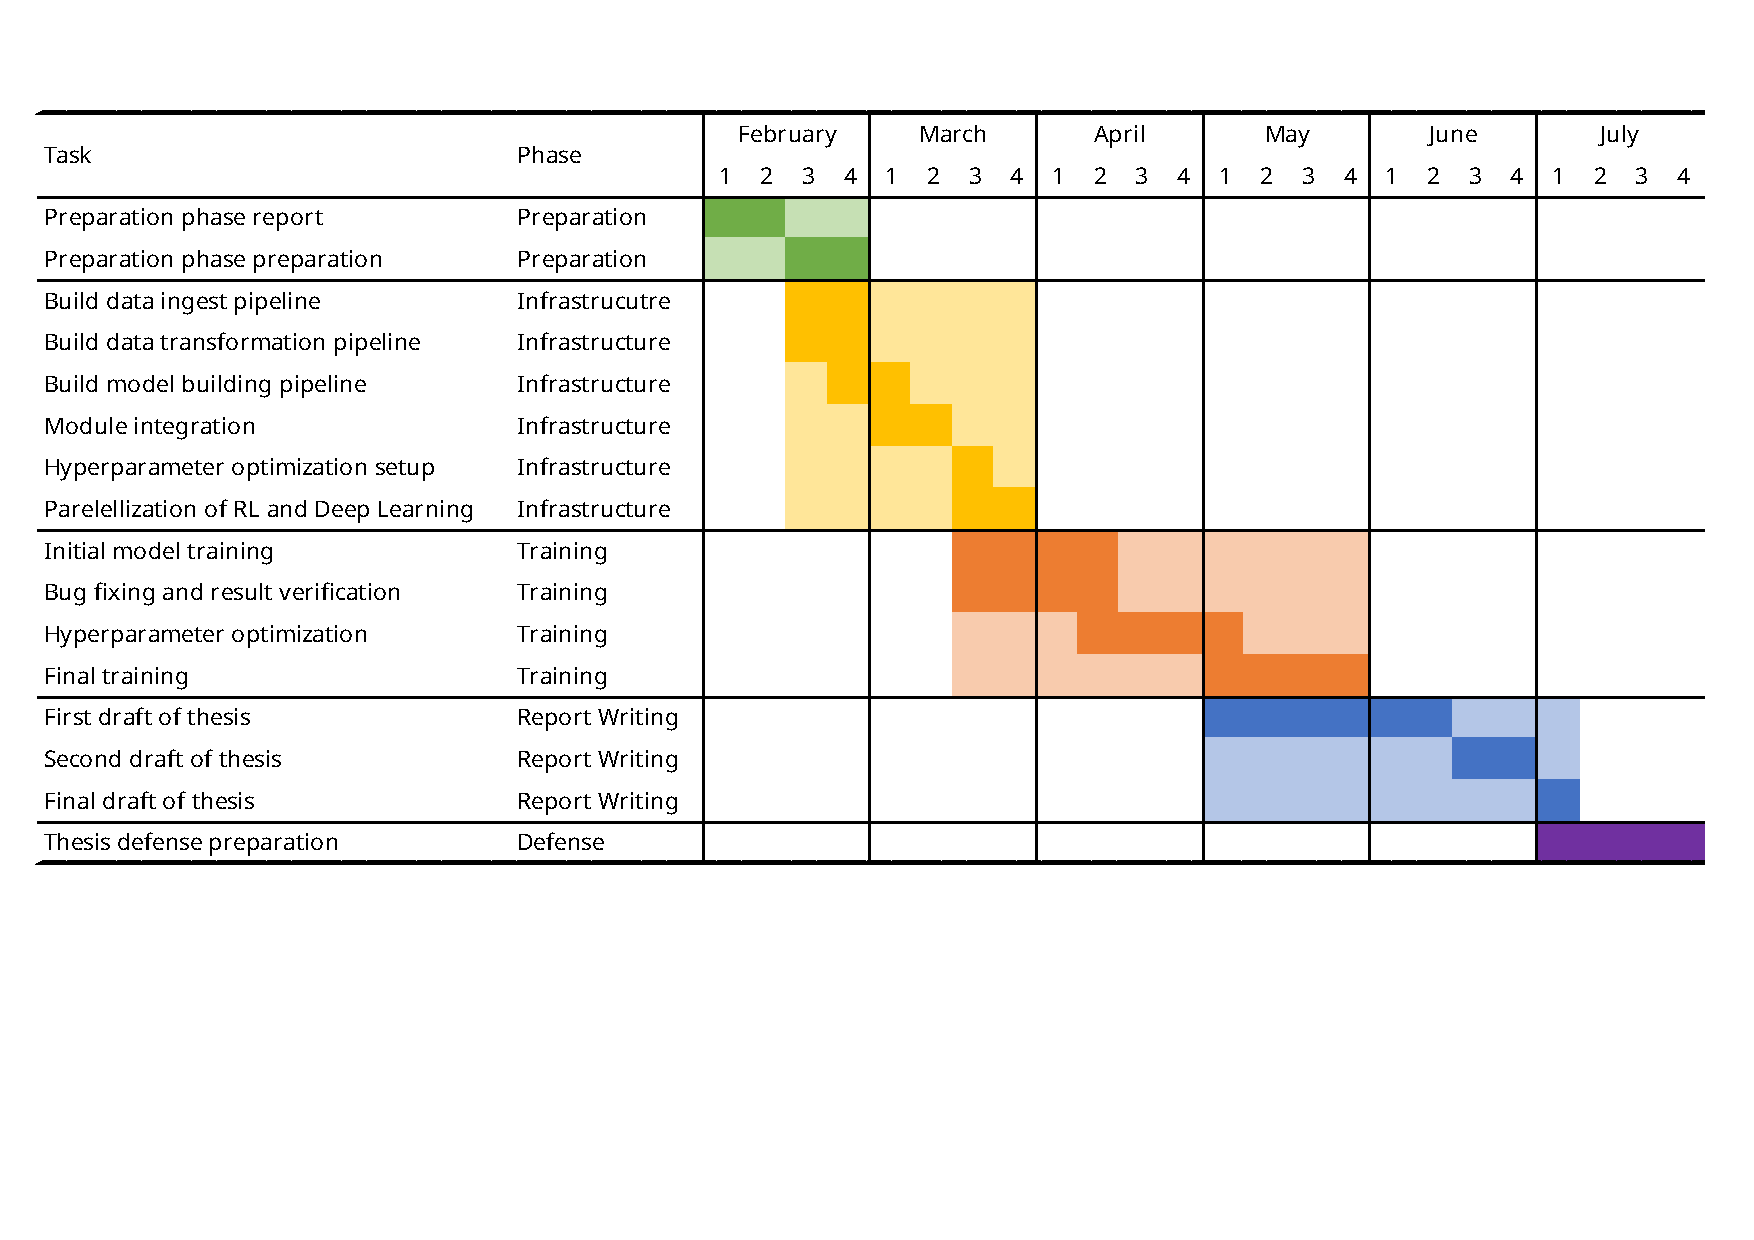
\includegraphics[width=\textwidth,trim={0.5cm 5cm 0.5cm 1cm},clip]{figures/gantt_chart}
	\caption{A Gantt chart showing the plan for this thesis}\label{fig:plan-gantt-chart}
\end{figure}